\documentclass{beamer}
\usetheme{Singapore}
\usecolortheme{default}

\usepackage[utf8]{inputenc}
\usepackage[T1]{fontenc}
\usepackage{verbatim}
\usepackage{graphics}
\usepackage{listings}
\usepackage{lmodern}

\title{Understanding Git with Alloy}
\subtitle{Milestone 2}
\author{Cláudio Lourenço \and Renato Neves}
\institute{University of Minho\\
Formal Methods in Software Engineering}


\logo{ 
\includegraphics[width=0.15\textwidth]{images/csail_logo.png}
       
\includegraphics[width=0.15\textwidth]{images/uminho_eng_logo.png}}

\begin{document}

\frame {
   \titlepage
}

\frame{
   \frametitle{Table of contents}
   \tableofcontents 
}

\section{Where were we?}
\frame{
   \frametitle{Where were we?}
         \begin{itemize}
            \item Focus on Index and Object Model
	    \item Ditched the Working Directory
            \item No problems with add and rm operations
            \item Big Problem in the commit
         \end{itemize}
}

\frame {
	\frametitle{What we are going to show}
		\begin{itemize}
			\item The solution to the commit problem 
			\item Heads up of the current model
			\item Show Commit, Add, Rm and Branch operations
			\item Focus on the Checkout operation
			\item Show some properties
			\item Future work
		\end{itemize}

}

\frame{
   \frametitle{The problem}
   \begin{figure}
      \centering
      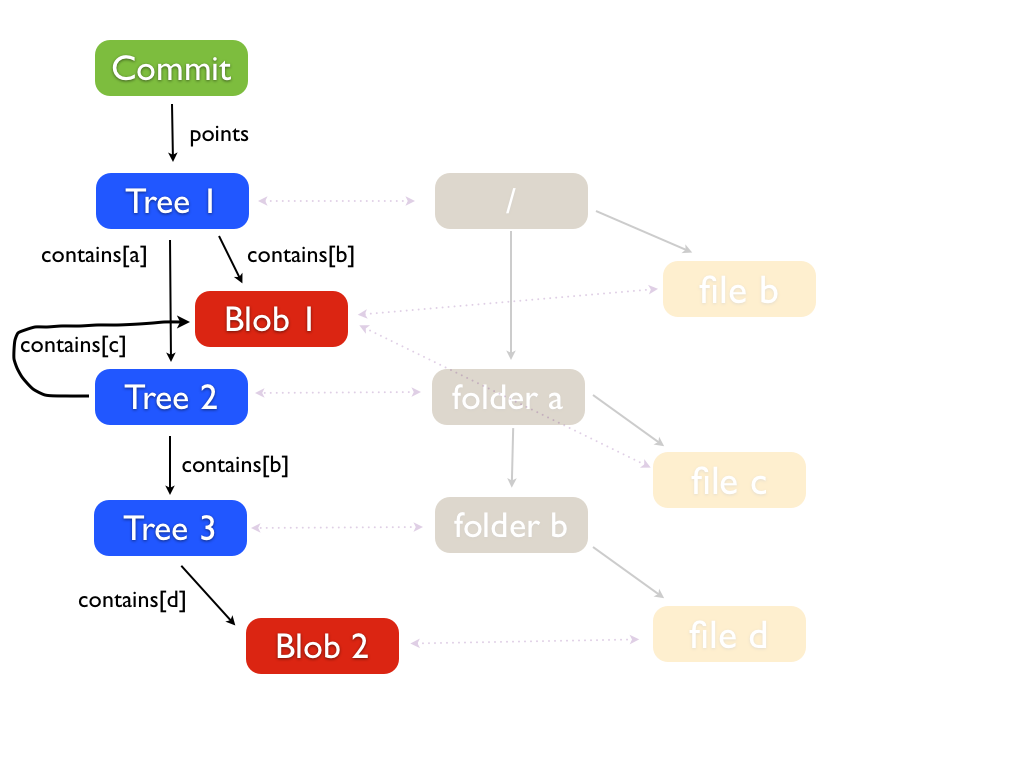
\includegraphics[width=0.7\textwidth]{images/CommitAbs1.png}
   \end{figure}
}

\frame {
	\frametitle{The problem}
	\begin{figure}
		\centering
		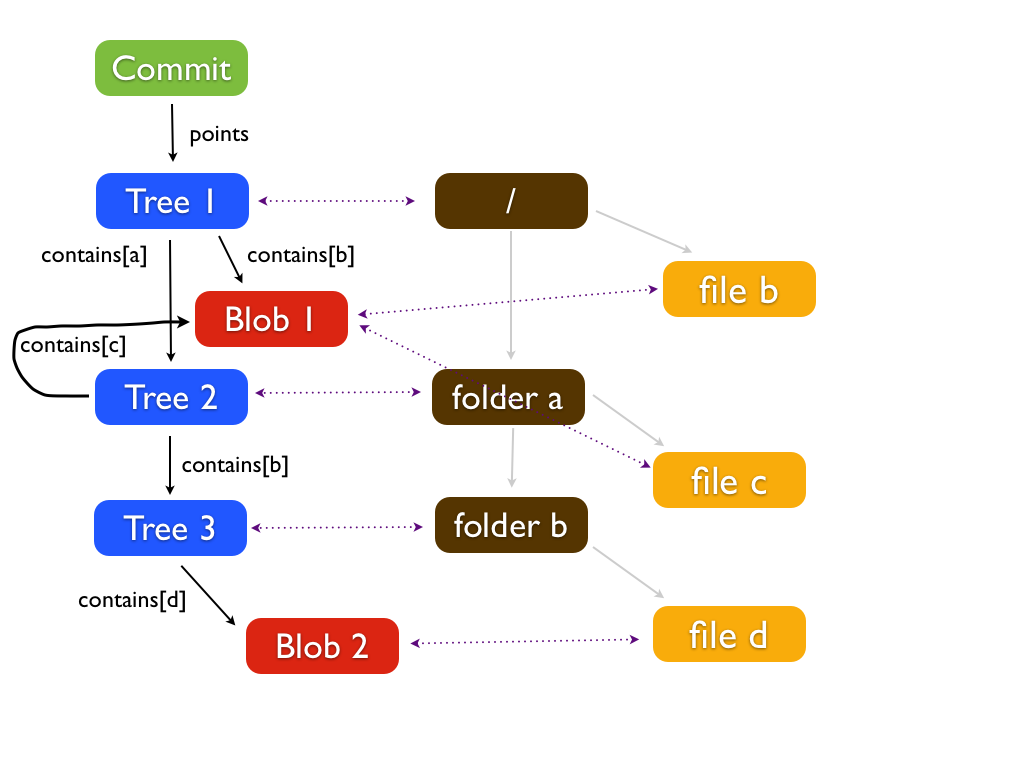
\includegraphics[width=0.7\textwidth]{images/CommitAbs2.png}
	\end{figure}
}

\frame {
	\frametitle{The problem}
	\begin{figure}
		\centering
		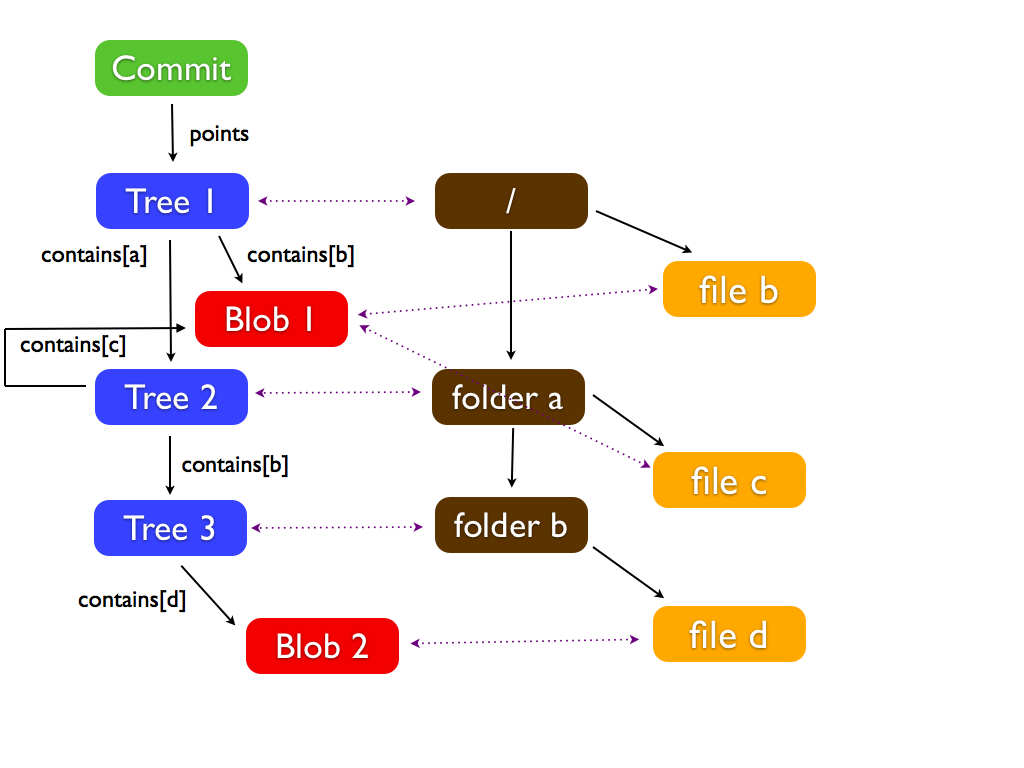
\includegraphics[width=0.7\textwidth]{images/CommitAbs3.png}
	\end{figure}
}

\section{Current Model}
\begin{frame}[fragile]
   \frametitle{Top view of the Model}
   \tiny
   \begin{columns}[c]
      \column{1.5in}
\begin{lstlisting}
sig Path {
   pathparent : lone Path,
   name : Name
}

sig File{
   path: Path,
   blob: Blob,
   index: set State
}
\end{lstlisting}
\color{blue}{
\begin{lstlisting}
abstract sig Object {
   objects: set State
}

sig Blob extends Object {}

sig Tree extends Object {
   contains : Name -> lone (Tree+Blob)
}

\end{lstlisting}
}
      \column{1.5in}
      \color{blue}{

\begin{lstlisting}

sig Commit extends Object {
   points : Tree,
   parent : set Commit,
   abs: Path -> Object
}

sig RootCommit extends Commit {}

sig Branch{
   marks: Commit one -> State,
   branches: set State,
   head: set State
}

lone sig Master extends Branch{}
                  
         \end{lstlisting}
      }
   \end{columns}
\end{frame}

\section{Progress}
\begin{frame}[fragile]
   \frametitle{Commit}
   \begin{block}{Abstraction}
      \begin{itemize}
         \item In each commit there is a relation between Objects and Paths
         \item Facts to reflect the parent relationship
            \begin{itemize}
               \item The Tree pointed by the Commit corresponds to the root
               \item A contains tuple exists, 
	       if and only if, the corresponding pathparent tuple exists
            \end{itemize}
      \end{itemize}
   \end{block}
   \tiny
   \begin{lstlisting}[escapechar=!]
                        sig Commit extends Object {
                           points : Tree,
                           parent : set Commit,
                           !\color{red}{abs: Path -> Object}!
                        }
  \end{lstlisting}

\end{frame}

\frame{
   \frametitle{The abstraction relation}
   \begin{figure}
      \centering
      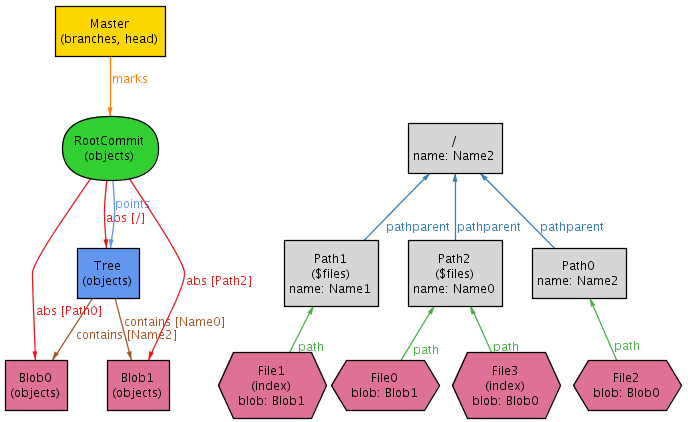
\includegraphics[width=0.8\textwidth]{images/abs2.png}
   \end{figure}

}

\begin{frame}[fragile]
   \frametitle{Operations - commit}
   \begin{block}{Commit}
      Creates a commit object, using the index as source information
   \end{block}
   \tiny
   \begin{block}{Commit Restrictions}
   	\begin{lstlisting}
	all p,q : (c.abs).univ | p -> q in pathparent => 
	q.(c.abs) -> p.(c.abs) -> p.name in contents
	...
	all t,o : objs, n : Name | t -> o -> n in contents => 
	all y : c.abs.t | some x : c.abs.o | x -> y in pathparent and x.name = n
	...
   \end{lstlisting}
	\end{block}
	\begin{block}{Commit Post Conditions}
	\begin{lstlisting}
	(head.s').(marks.s').parent = (head.s).(marks.s)
	...
	(index.s).path.*pathparent = (head.s').(marks.s').abs.univ
	all f:index.s | f.path -> f.blob in (head.s').(marks.s').abs
	...
   	\end{lstlisting}
	\end{block}
\end{frame}

\begin{frame}[fragile]
   \frametitle{Operations - commit}
   \begin{figure}
      \centering
      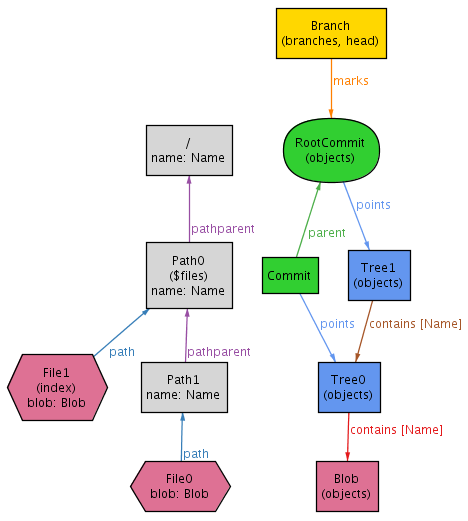
\includegraphics[width=0.5\textwidth]{images/commit1.png}
   \end{figure}
\end{frame}

\begin{frame}[fragile]
   \frametitle{Operations - commit}
   \begin{figure}
      \centering
      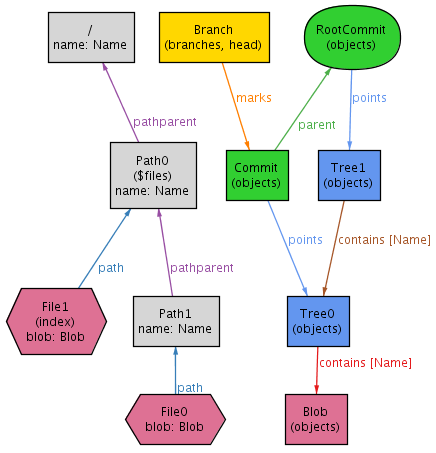
\includegraphics[width=0.5\textwidth]{images/commit2.png}
   \end{figure}
\end{frame}


\section{The operations}
\begin{frame}[fragile]
   \frametitle{Operations - add and rm}
   \begin{block}{add}
      Add a file with the current content to the index
   \end{block}
   \tiny
   \begin{lstlisting}
...
index.s' = index.s + f - ((f.path).~path -f)
   \end{lstlisting}
   \normalsize
   \begin{block}{rm}
      Remove the file from the index
      \begin{itemize}
	\item The file must exist in the index
	\item The file with its content must exist in the current commit
	\item If you add a file, you can only remove it after committing it 
      \end{itemize}
   \end{block}
   \tiny
   \begin{lstlisting}
...
f in index.s
f.path -> f.blob in (head.s).(marks.s).abs
...
index.s' = index.s - f
   \end{lstlisting}
\end{frame}


\begin{frame}[fragile]
   \frametitle{Operations - branch}
   \begin{block}{branch}
      Creates a new branch pointing to the current commit
   \end{block}
   \tiny
   \begin{lstlisting}
...
branches.s' = branches.s + b
marks.s' = marks.s + b -> (head.s).(marks.s)
...
   \end{lstlisting}
   \normalsize
   \begin{block}{branch -d}
      Removes a branch if it is not pointed by the head.
      Also it's information must be achieved by the 
      current branch
   \end{block}
   \tiny
   \begin{lstlisting}
...
b not in (head.s)
b.marks.s in (head.s).(marks.s).*parent
...
branches.s' = branches.s - b
marks.s' = marks.s - b -> Commit
...
   \end{lstlisting}
\end{frame}

\begin{frame}[fragile]
   \frametitle{Operations - branch}
   \begin{columns}[c]
      \column{1.5in}
      \begin{figure}
         \centering
         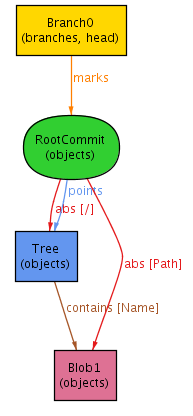
\includegraphics[width=0.75\textwidth]{images/branch1.png}
      \end{figure}
      \pause
      \column{1.5in}
      \begin{figure}
         \centering
         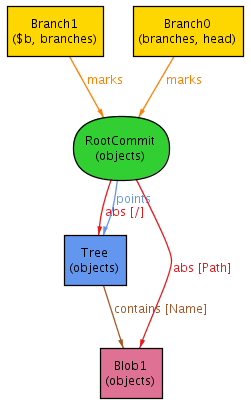
\includegraphics[width=0.90\textwidth]{images/branch2.png}
      \end{figure}
   \end{columns}
\end{frame}

\begin{frame}[fragile]
   \frametitle{Operations - checkout}
	 "...It adds, removes, and modifies files automatically to make 
	 sure your working copy is what the branch looked like on your last commit to it."	 
	 \footnote{Git Community Book}
	\pause
   \begin{block}{Problems}
      \begin{itemize}
         \item There are no specifications
	 \item Difficulty to understand the pre-conditions
	 \item "if there are any uncommitted changes when you run git checkout,
	 Git will behave very strangely." \footnote{Understanding Git}
	\end{itemize}
   \end{block}
\end{frame}

\begin{frame}
   \frametitle{Checkout}
   \begin{block}{Pre-conditions found}
      Everything that is in the index has to be in the current commit with the
      same content, except if:
      \begin{itemize}
         \item The content of a file is the same in the
         current and destination commit - in this case
         the file in the index keeps its content (warning is thrown)
         \item Exists a file in the index, and that file does not exists
         neither in the current nor in the destination commit - in
         this case the file is kept in the index (warning is thrown)
         \item Content of the file in the index is the same as in the
         destination commit (no warning is thrown)
      \end{itemize}
   \end{block}
\end{frame}

\begin{frame}[fragile]
   \frametitle{Checkout - Alloy}
	\tiny
	\begin{lstlisting}
   ...
   let CA = (head.s).(marks.s).abs :> Blob, 
       IA = s.pathcontents,
       CB = (b.marks.s).abs :> Blob
   ...
	\end{lstlisting}
   \pause
	\begin{lstlisting}
   
   all f:index.s | f.path -> f.blob in (IA - CA) 
                   => (f.path in CB.univ 
                        => (f.path -> f.blob in CB or (f.path).CA = (f.path).CB)
                        else f.path not in CA.univ)
   ...
	\end{lstlisting}
   \pause
	\begin{lstlisting}
   
   s'.pathcontents = CB ++ (IA - CA)
   ...
   \end{lstlisting}
\end{frame}


\begin{frame}[fragile]
   \frametitle{Checkout - Instance 1}
      \begin{figure}
         \centering
         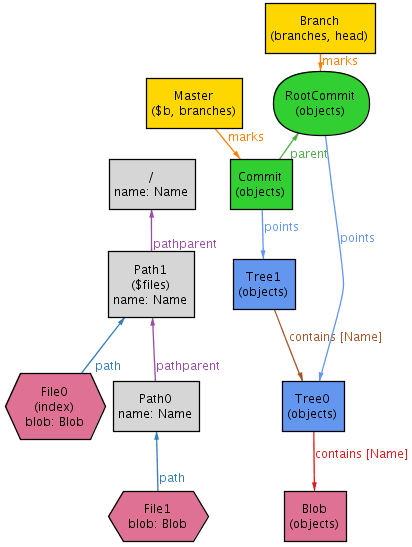
\includegraphics[width=0.50\textwidth]{images/checkout1.png}
      \end{figure}
\end{frame}

\begin{frame}[fragile]
   \frametitle{Checkout - Instance 1}
      \begin{figure}
         \centering
         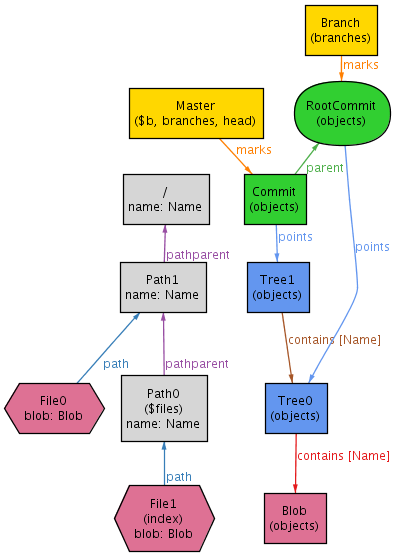
\includegraphics[width=0.50\textwidth]{images/checkout2.png}
      \end{figure}
\end{frame}

\begin{frame}[fragile]
   \frametitle{Checkout - Instance 2}
      \begin{figure}
         \centering
         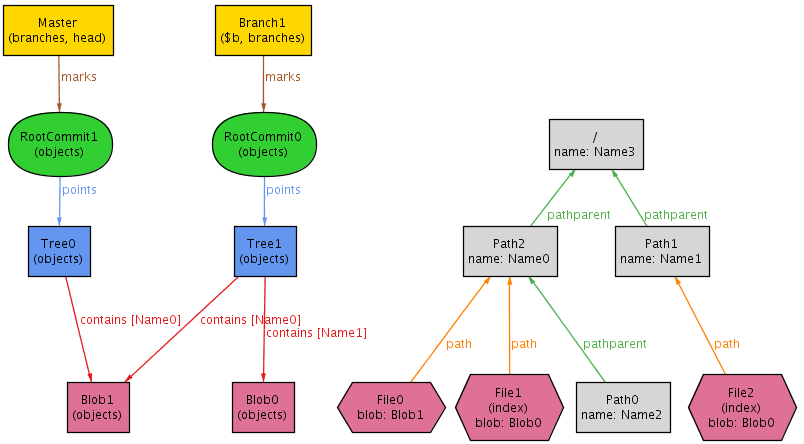
\includegraphics[width=0.80\textwidth]{images/checkout2_1.png}
      \end{figure}
\end{frame}

\begin{frame}[fragile]
   \frametitle{Checkout - Instance 2}
      \begin{figure}
         \centering
         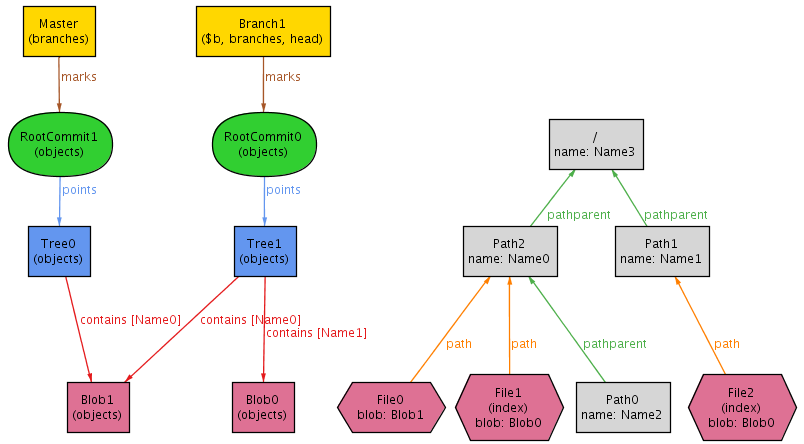
\includegraphics[width=0.80\textwidth]{images/checkout2_2.png}
      \end{figure}
\end{frame}

\begin{frame}
	\frametitle{Checkout - Bug}
	\begin{itemize}
	   \item touch f \pause
	   \item git add f \pause
	   \item git commit \pause
	   \item git rm f \pause
	   \item mkdir f \pause
	   \item touch f/g \pause
	   \item git add f/g \pause 
	   \item git checkout b 
	\end{itemize}
\end{frame}

\begin{frame}
   \frametitle{Why we assume it is a bug} \pause
   \begin{block}{Git Mailing list}
      \footnotesize
      \begin{itemize}
         \item ''I think providing a link to that "alloy" thing could
         be helpful.'' \pause
         \item ''When you create a branch, it will contain everything
         committed on the branch you created it from at that given
         point. So if you commit more things on the master branch like
         you have done (after creating b), then switch to branch b,
         they won't appear. This is the correct behavior. Does that
         answer your question?'' \pause
         \item ''Yes, that looks like a bug. Checkout should not
         overwrite uncommitted files. It does the right thing if you
         do not "git add f/g" (it complains that deleting the
         directory would lose untracked files). But if the file has
         been added to the index, we seem to miss the check.''
      \end{itemize}
   \end{block}
\end{frame}

\section{The properties}
\begin{frame}[fragile]
   \frametitle{Properties}
   \begin{block}{Invariant preservation}
      All operations must preserve the invariant
   \end{block}
   \vspace{0.1in}
   \scriptsize
all s,s':State,... | invariant[s] and operation[s,s',...] => invariant[s'] \\
   \normalsize
   \vspace{0.1in}
   \begin{itemize}
      \item There is some commit iff exists at least one branch and
      an head
      \item The current branch must exist and must have a commit
      \item All objects from one state descend from one of its commits
      \item Referential integrity is kept on dynamic relations
      \item There are no empty trees
   \end{itemize}

\end{frame}

\begin{frame}[fragile]
   \frametitle{Properties}
   \begin{block}{Idempotence}
      \begin{itemize}
         \item After performing an operation, repeating it does not change the state
         \item Add, commit and checkout are idempotent
      \end{itemize}
   \end{block}
   \scriptsize
   \begin{lstlisting}
	all s0,s1,s2 : State | 
		operation[s0,s1,...] and operation[s1,s2,...] => 
		   dynamicRelations[s1] = dynamicRelations[s2]
   \end{lstlisting}
\end{frame}

\begin{frame}[fragile]
	\frametitle{Properties}
	\begin{block}{Commit, Add, Commit, Rm, Commit}
	\begin{itemize}
		\item Resulting from this sequence of operations, the last
		commit must be equal to the first commit
	\end{itemize}
	\end{block}
	\scriptsize
	\begin{lstlisting}
	all s0,s1,s2,s3,s4,s5:State, f:File | 
  
        commit[s0,s1] 
        and add[s1,s2,f] 
        and f.path not in (index.s1).path 
        and commit[s2,s3] 
        and rm[s3,s4,f] 
        and commit[s4,s5]
	
   => ((head.s1).(marks.s1).points = (head.s5).(marks.s5).points)
	\end{lstlisting}
	\normalsize
\end{frame}

\begin{frame}[fragile]
	\frametitle{Properties}
	\begin{block}{Revert the Checkout}
	\begin{itemize}
		\item If we checkout to a given branch, and then checkout to the
		branch where we were, the commit and index before the first checkout must
		be the equal to the commit and index after the second checkout. In other
		words, no changes in the state
	\end{itemize}
	\end{block}
	\scriptsize
	\begin{lstlisting}
all s,s',s'':State, b:Branch | 
   checkout[s,s',b] and checkout[s',s'',head.s] => 
      (head.s).(marks.s) = (head.s'').(marks.s'') 
      and s.pathcontents = s''.pathcontents
	\end{lstlisting}
	\normalsize
\end{frame}

\begin{frame}[fragile]
	\frametitle{Properties}
	\begin{block}{Checkout, all files from commit will be in index}
      When a checkout is performed, all files that are on the commit
      pointed by b, will be in the index.
   \end{block}
	\scriptsize
	\begin{lstlisting}
all s,s':State, b:branches.s, p:Path, blo:Blob | 
      p->blo in (b.marks.s).abs => some f:File | 
         f.path = p and f.blob = blo and f inindex.s'
	\end{lstlisting}\pause
   \Large
   \color{red}
   \center
   Counter Examples found
\end{frame}

\section{Future work}
\frame{
   \frametitle{Future work}
   \begin{itemize}
      \item Finish the Merge operation (used for Push and Pull)
      \item Add more interesting properties
      \item Maybe try to model git rebase
      \item Document operations and properties
   \end{itemize}
}


\frame{
   \titlepage
}

\end{document}
